
\section{Preprocessing}

\subsection{Data}

The samples are real VBC calls that were made between 1.1.2018 to 22.1.2018, and that were rated by an iOS user. Each call is represented by # feature, and has label (y) - which is the call's rate.

The calls were retrieved from Kibana (Elastic search). The matched rates are taken from Localytics.

\paragraph{Rates}\label{Rates}

The Rated


\section{Analysis}

\subsection{1. Impairments vs Rating analysis}

The analysis phase's goal was to evaluate the separability of star classes based on the features collected for each sample.
most of the work was exploratory and contained visualization of segements of the deta in different forms to highlight change in distributions as function of change in feature/s

Figures  \ref{fig:mos_vs_stars} presents the distributions of different quality measures as a function of the Rate. The box plots in those figures shows that for lower rates the there are more samples with "bad" levels of quality measures than in high rates.
This insight suggest a relation between quality and rates that supplied the required justification to keep exploring in that direction.
In spite of the suggested direction by those figures , few notes most taken into account :
1. The charts hides out-liners ( lower 2.5\% , upper 2.5 \%) . because of the unbalanced distribution of rates, the out liners of the high Rates are mixed "overlay" the significance of the difference 
2. Most of the population of the Rates groups lays around the same values so the segregation suggested by the box plot distribution is only effective to extreme cases 

Sample of the distributions are presented below :

\paragraph{Rates vs. MOS}\label{rates-vs.-jitter}

As we can see, lower MOS values tend to appear in calls that were rated
as bad calls.

\begin{center}
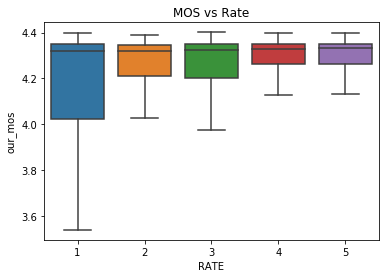
\includegraphics{figures/output_23_0.png}
\end{center}

\paragraph{Rates vs. jitter}\label{rates-vs.-jitter}

High jitter average values tend to appear in calls that were rated as
bad calls.

\begin{center}
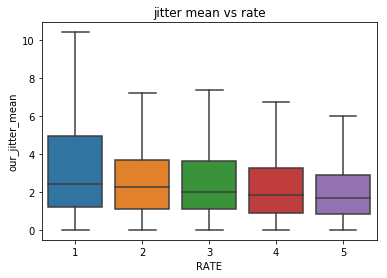
\includegraphics{figures/output_25_0.png}
\end{center}
    
\paragraph{Rates vs. RTT (latency)}\label{rates-vs.-rtt-latency}

High RTT average values tend to appear in calls that were rated as bad
calls.

 


\begin{center}
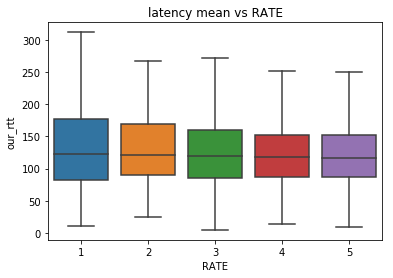
\includegraphics{figures/output_27_0.png}
\end{center}

    
\paragraph{Rates vs. Packet lost}\label{rates-vs.-packet-lost}

High packet lost percentage values tend to appear in calls that were
rated as bad calls.




\begin{center}
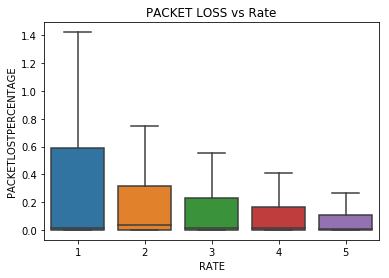
\includegraphics{figures/output_29_0.png}
\end{center}
    
\subsubsection{2. Call length}\label{call-length}

Another Promising dimension is the call length. we hypothesize that quality calls will be over earlier than that similar calls that have good quality. if indeed this assumption is current and also our basic thesis about the quality and Rates correlation  

\begin{center}
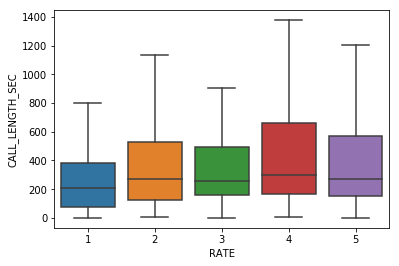
\includegraphics{figures/output_32_0.png}
\end{center}


\subsubsection{}



\subsubsection{Subsection}




% %-------------------------Content------------------------
